\documentclass{neu_handout}
\usepackage{url}
\usepackage{amssymb}
\usepackage{amsmath}
\usepackage{marvosym}
\usepackage{graphicx}
\usepackage[pdftex]{graphicx}
\usepackage{subfigure}
\graphicspath{ {images/} }
\everymath{\displaystyle}


% Professor/Course information
\title{Homework 1 - Part 3}
\author{Emily Dutile}
\date{January 2018}
\course{CS7295}{Info Viz}

\begin{document}


\section*{Who is CS7295}

\subsection*{2. Data Types}

\begin{center}
Table 1: Data Types
\end{center}
\begin{center} 
\begin{tabular}[h]{l l l l}
\textbf{Column} & \textbf{Data Type} \\
City & categorical \\
Country & categorical \\ 
State & categorical \\
Native language & categorical \\
Languages known other than English & categorical \\
Preferred OS & categorical \\
Mobile OS & categorical \\
Favorite language & categorical \\
Chocolate or Vanilla & categorical \\
Preferred OS & categorical \\
Color & categorical \\
Favorite number & quantitative \\
Temperate & quantitative \\
Amount of coffee & quantitative \\
Wake up & quantitative \\
To bed & quantitative \\
Visual encoding & category
\end{tabular}
\end{center}

\subsection*{4. Data Clean-Up}
To clean up the data, the data was exported to a new excel spreadsheet. Column names were shortened for readability, categorical data was made the same (i.e.: USA vs. United States), null values were filled with None or NA, verbose answers were shorted, state abbreviations were spelled out, string values were capitalized, degrees were converted to Farenheight if necessary, exclamation points were removed, and numbers that were spelled out were made quantitative.\\

If this was a much larger data set, I would have wrote a web crawler in python using the BeautifulSoup library to extract the html and parse the desired text. Since there is no student name in the original dataset, joining would be difficult without a given key, so this step would be kept manual for sake of time.

\subsection*{6. Data Gathering}
From Piazza I compared the information hints as to what text blurb matched with the data in the csv. I simply inserted two rows for department (CCIS or other) and what degree program the individual is pursuing. There wasn't a great deal of cleaning the data here.

\subsection*{7. Questions}

\subsubsection*{7.1}
Is there a correlation between bedtime and coffee consumption? Please see Appendices for visual.\\

There seems to be a slight correlation between individuals that go to bed late at night (or very early in the morning) and the amount of coffee consumed. Overall, it appears that individuals who go to bed earlier at night seem to consume less coffee.\\

I chose to use a scatter plot to show the individual points on the horizontal and vertical channel with a blue circle mark. The plot ranges from 12AM to 11PM EST.

\subsubsection*{7.2}
Is there a typical “profile” for someone who prefers to use a mobile phone with an Android versus Apple OS?\\

It appears that if you prefer Apple iOS for your mobile device, there's a strong chance that you prefer/use Apple OS as well. The results are biased towards students in the US since there are more US students in the data. If you prefer Android, you probably prefer Windows (Linux/Unix is close). Both profiles seems to prefer python as well.

\subsection*{8. Additional Questions and Visualizations}


\subsubsection*{8.1}

What parts of the world do the students of CS7295 represent?\\

I chose to use a map in order to visualize the areas in which students come from. I thought that using anything more than one color would add undesired interpretation since I am simply illuminating parts of the world where students are from.


\subsubsection*{8.2}
What are students favorite color? \\

I thought that utilizing an area chart would easily show the popularity of colors (by mark and channel). Making each box based on the actual color made it quicker to read at a glance, rather than using simply text.


\subsubsection*{8.3}
What percentage of students are bilingual? Please see Appendices for visual.\\

I chose to use a pie chart with 2 attributes encoded, area and color in order to show the number of bilingual students in the class. The angle easily shows that nearly 75\% of the class is bilingual.

\newpage

\appendix
\section{Appendices}

\begin{figure}[h]
\centering
{
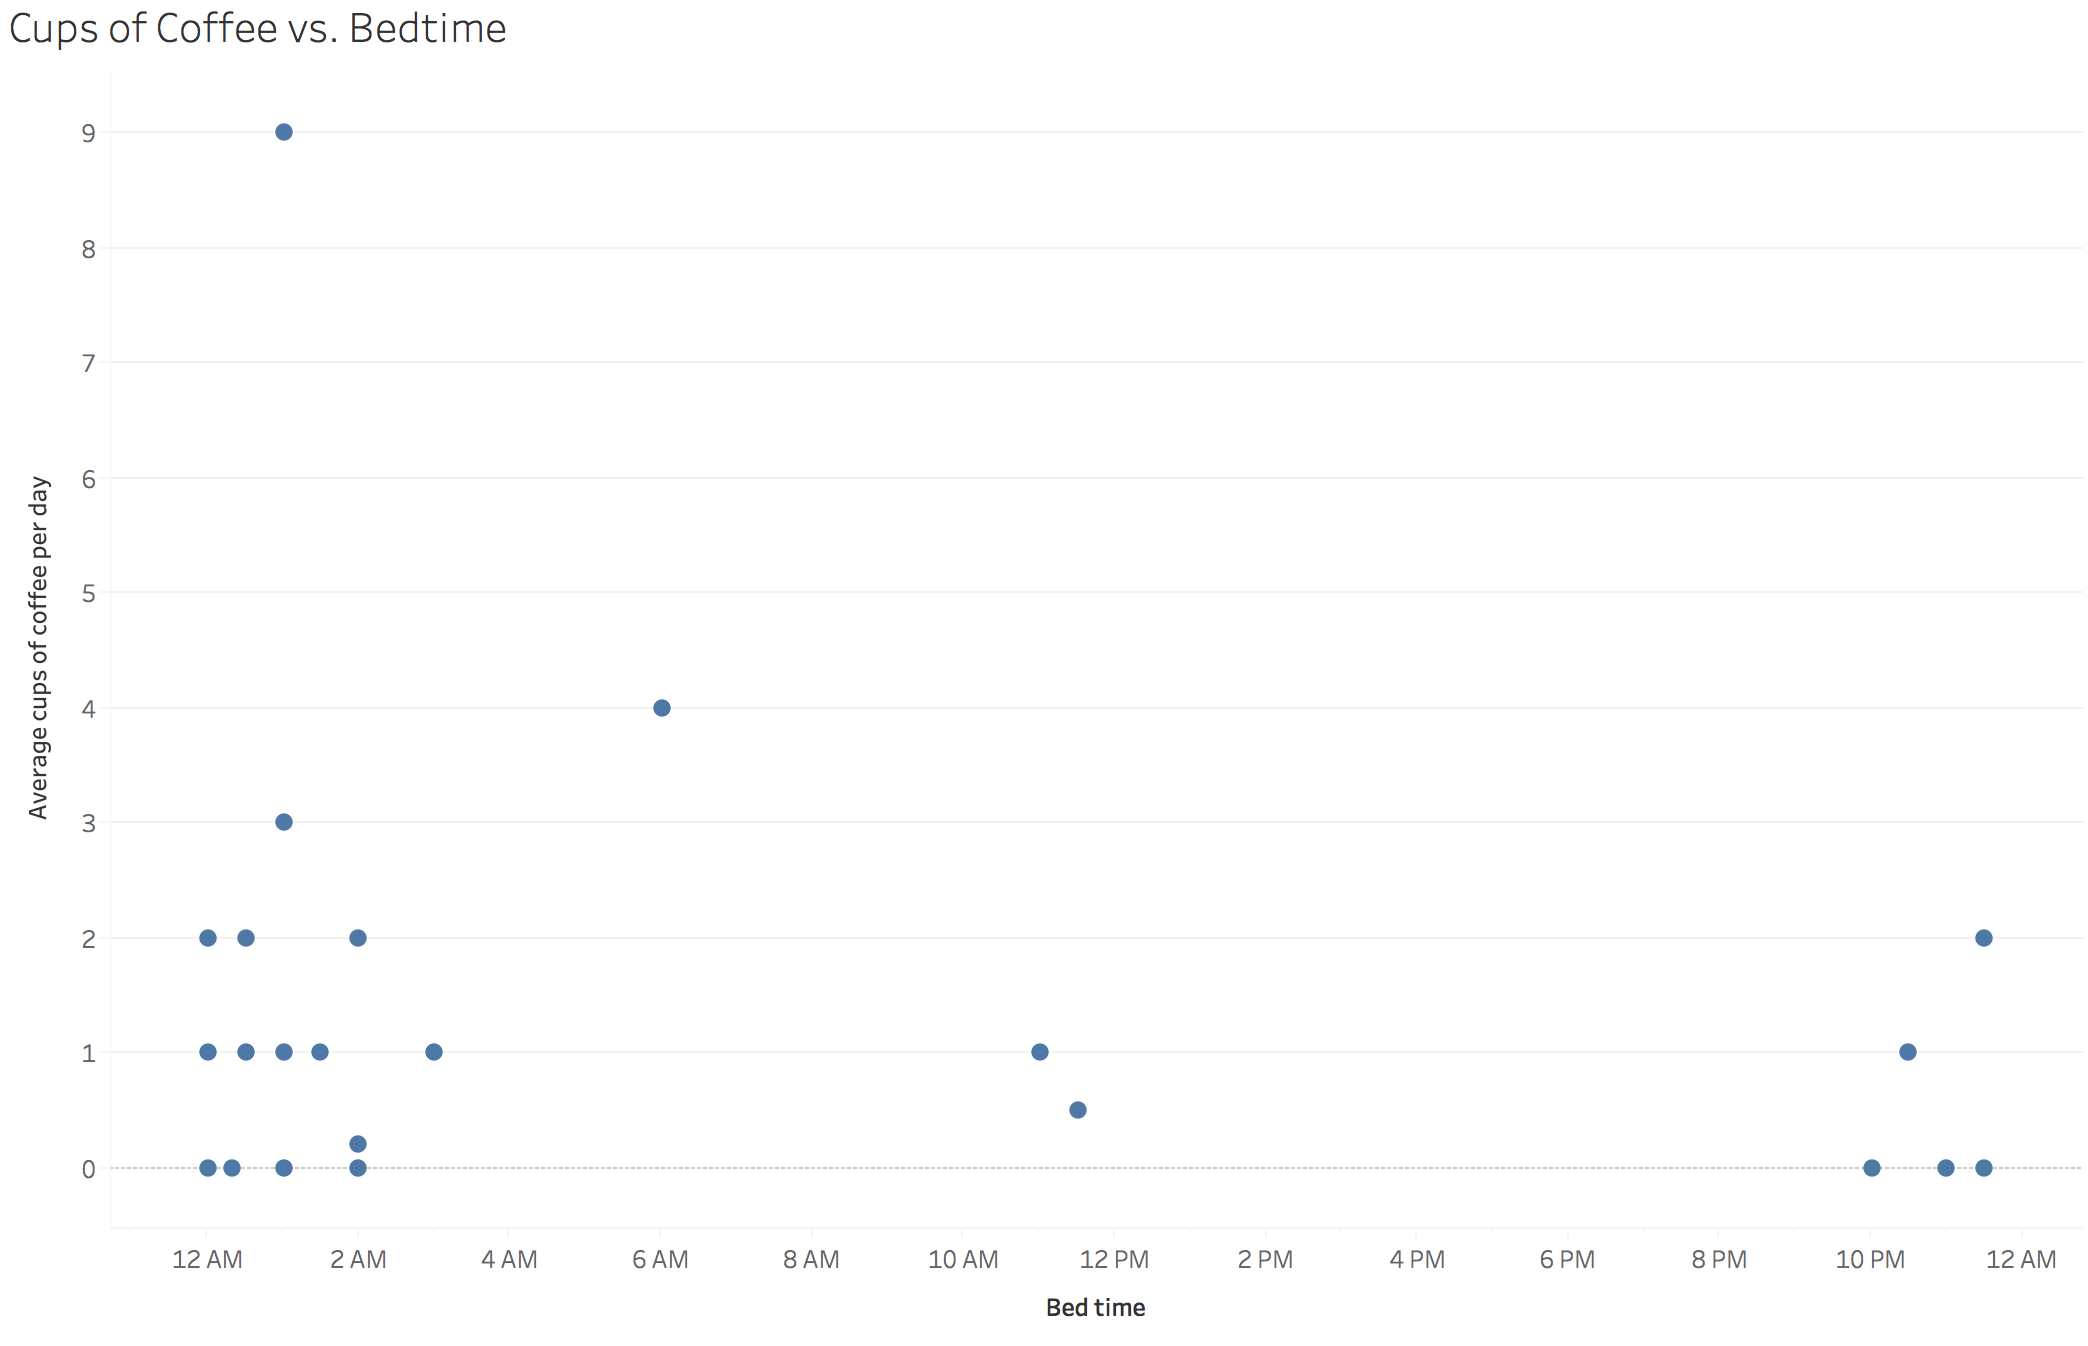
\includegraphics[width=0.7\linewidth]{coffeevsbedtime}
}
\end{figure}

\begin{figure}[h]
\centering
{
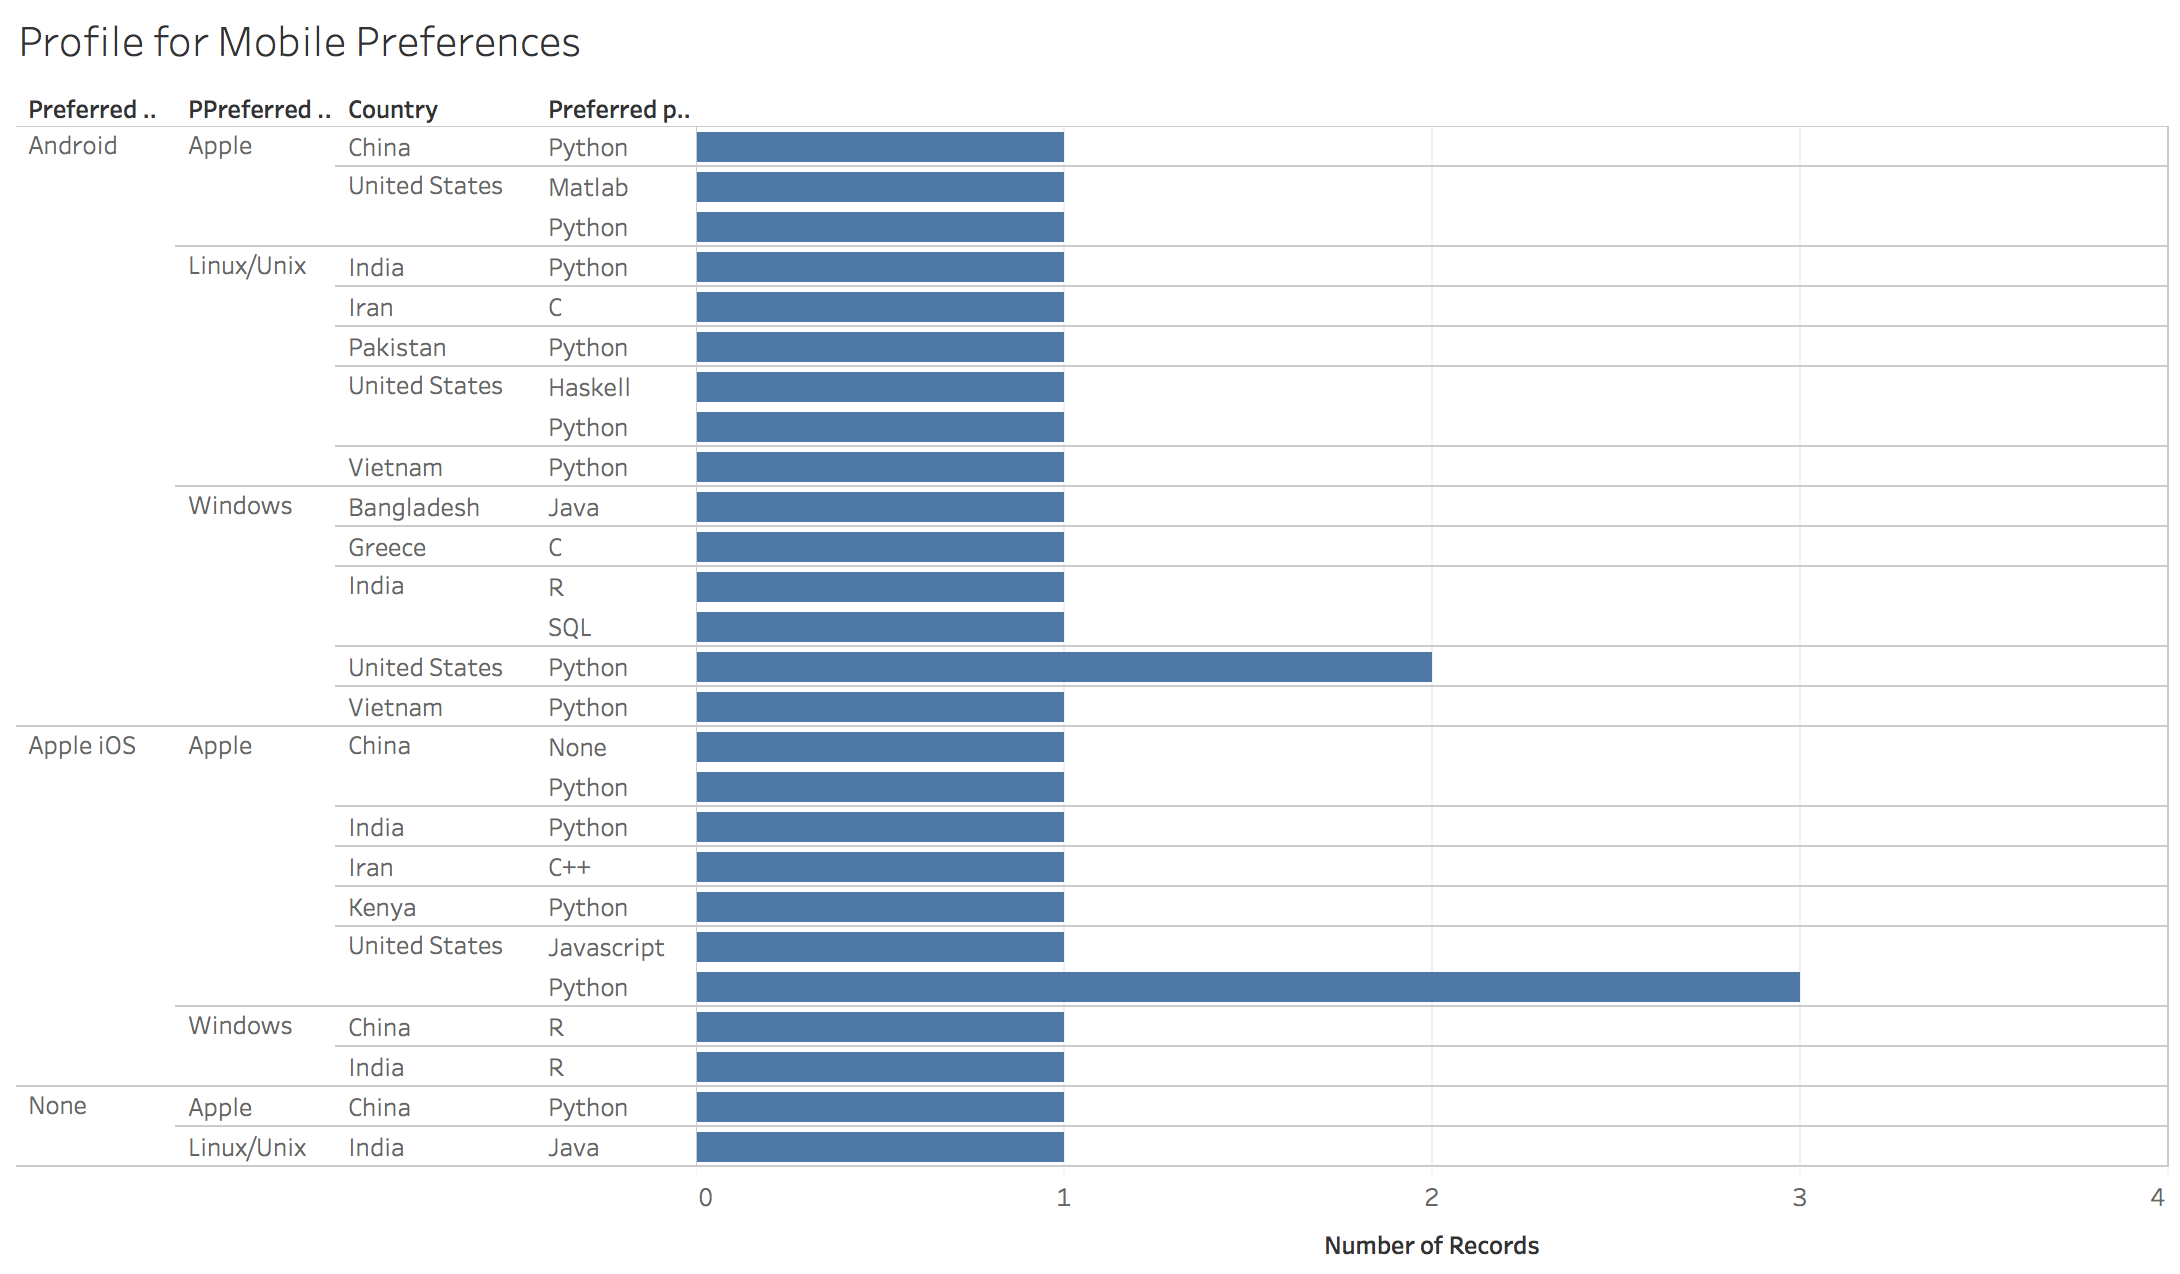
\includegraphics[width=0.7\linewidth]{profile}
}
\end{figure}


\begin{figure}[h]
\centering
{
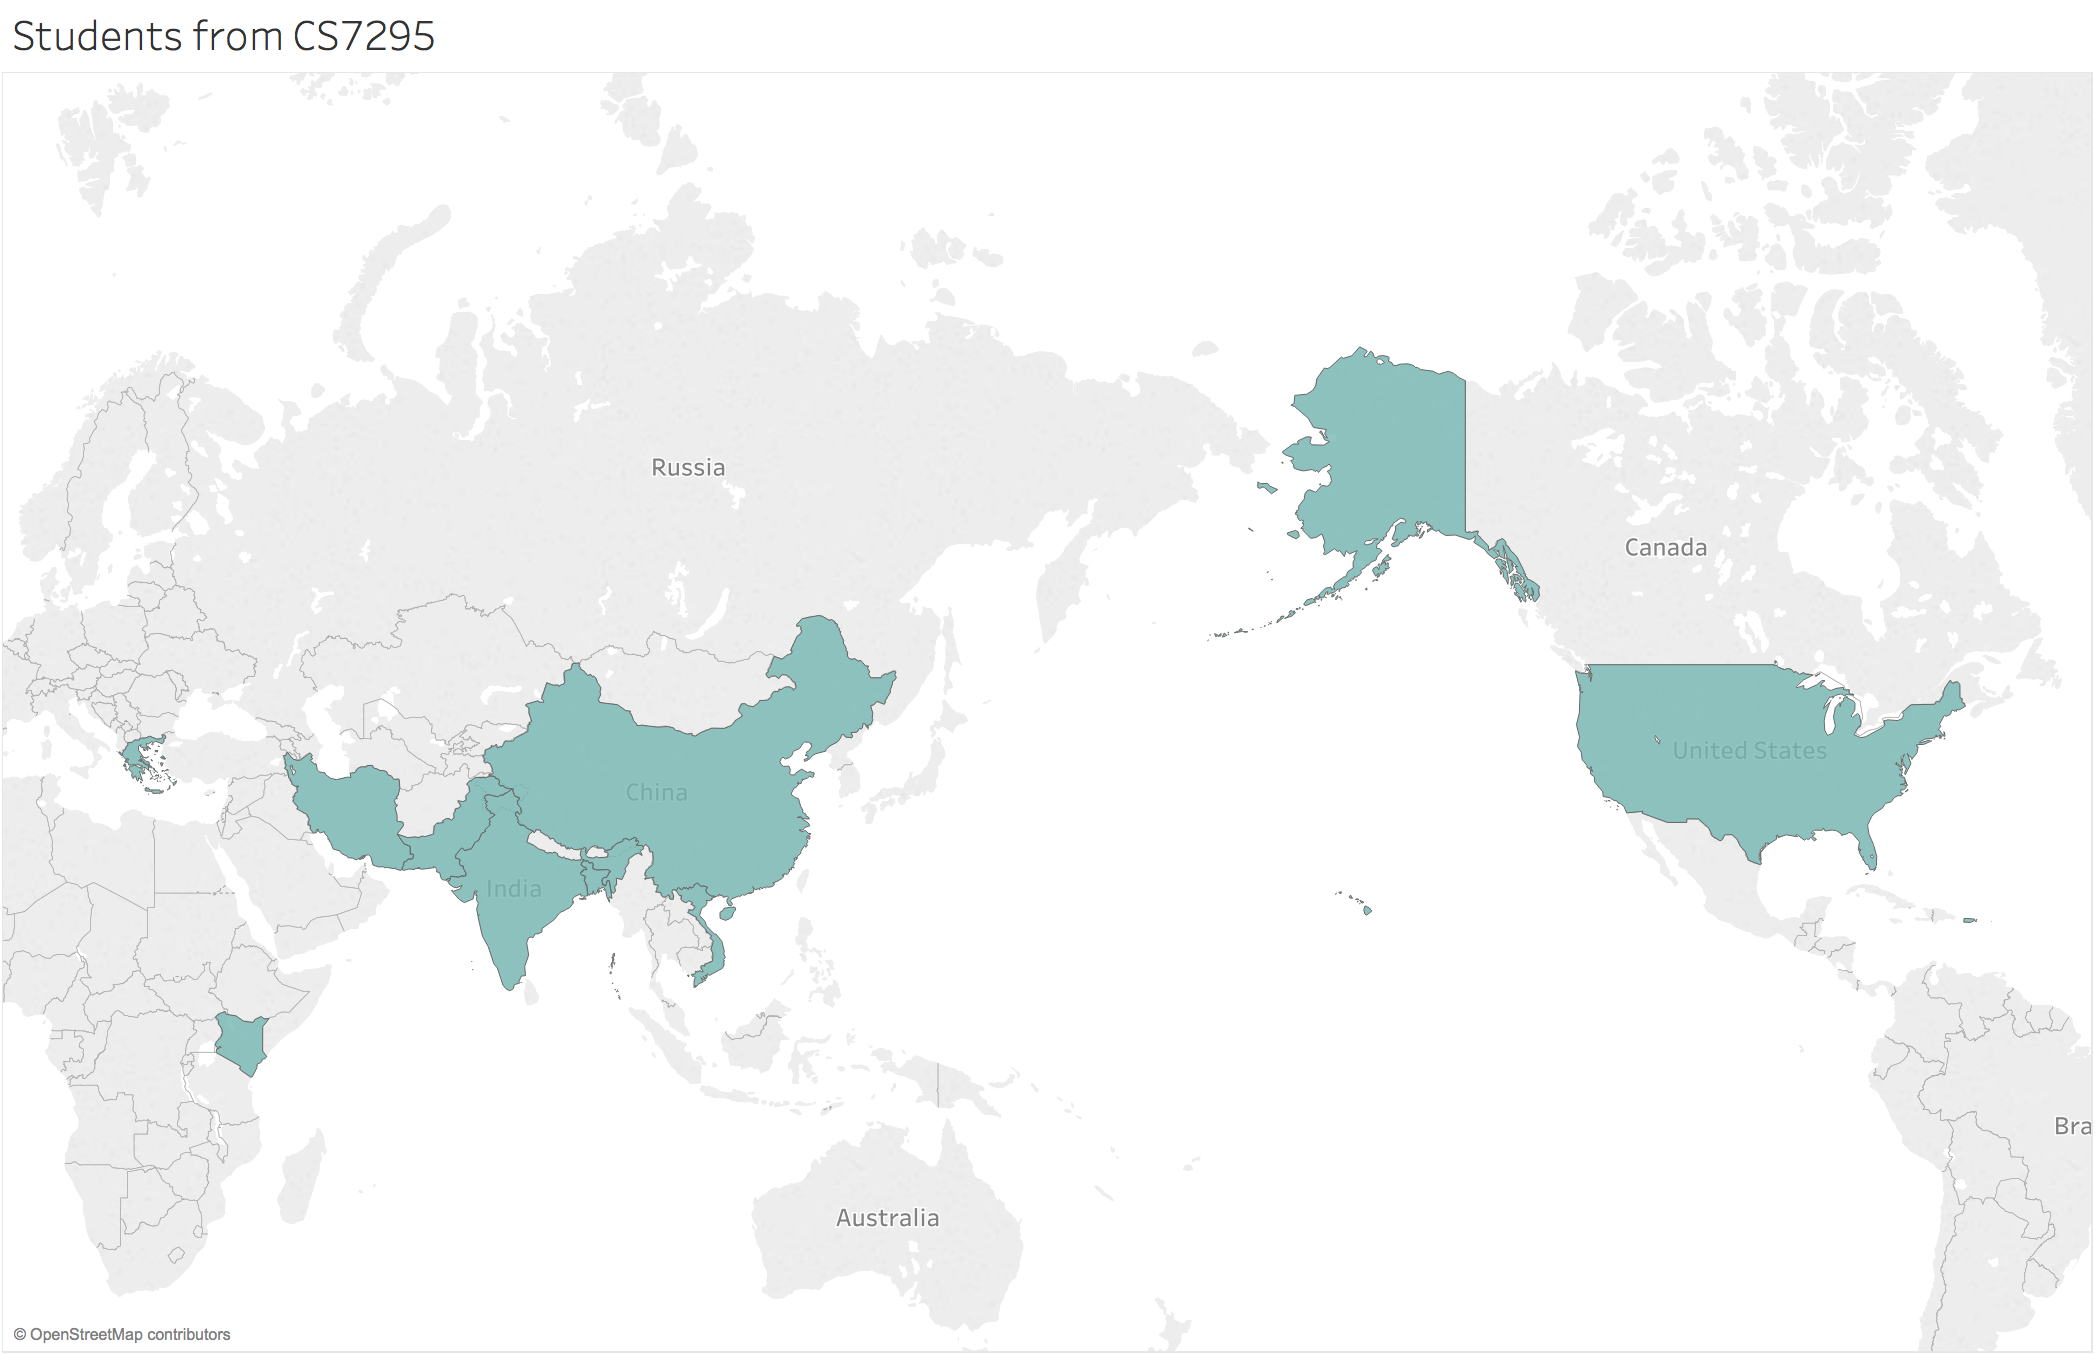
\includegraphics[width=0.7\linewidth]{map}
}
\end{figure}

\begin{figure}[h]
\centering
{
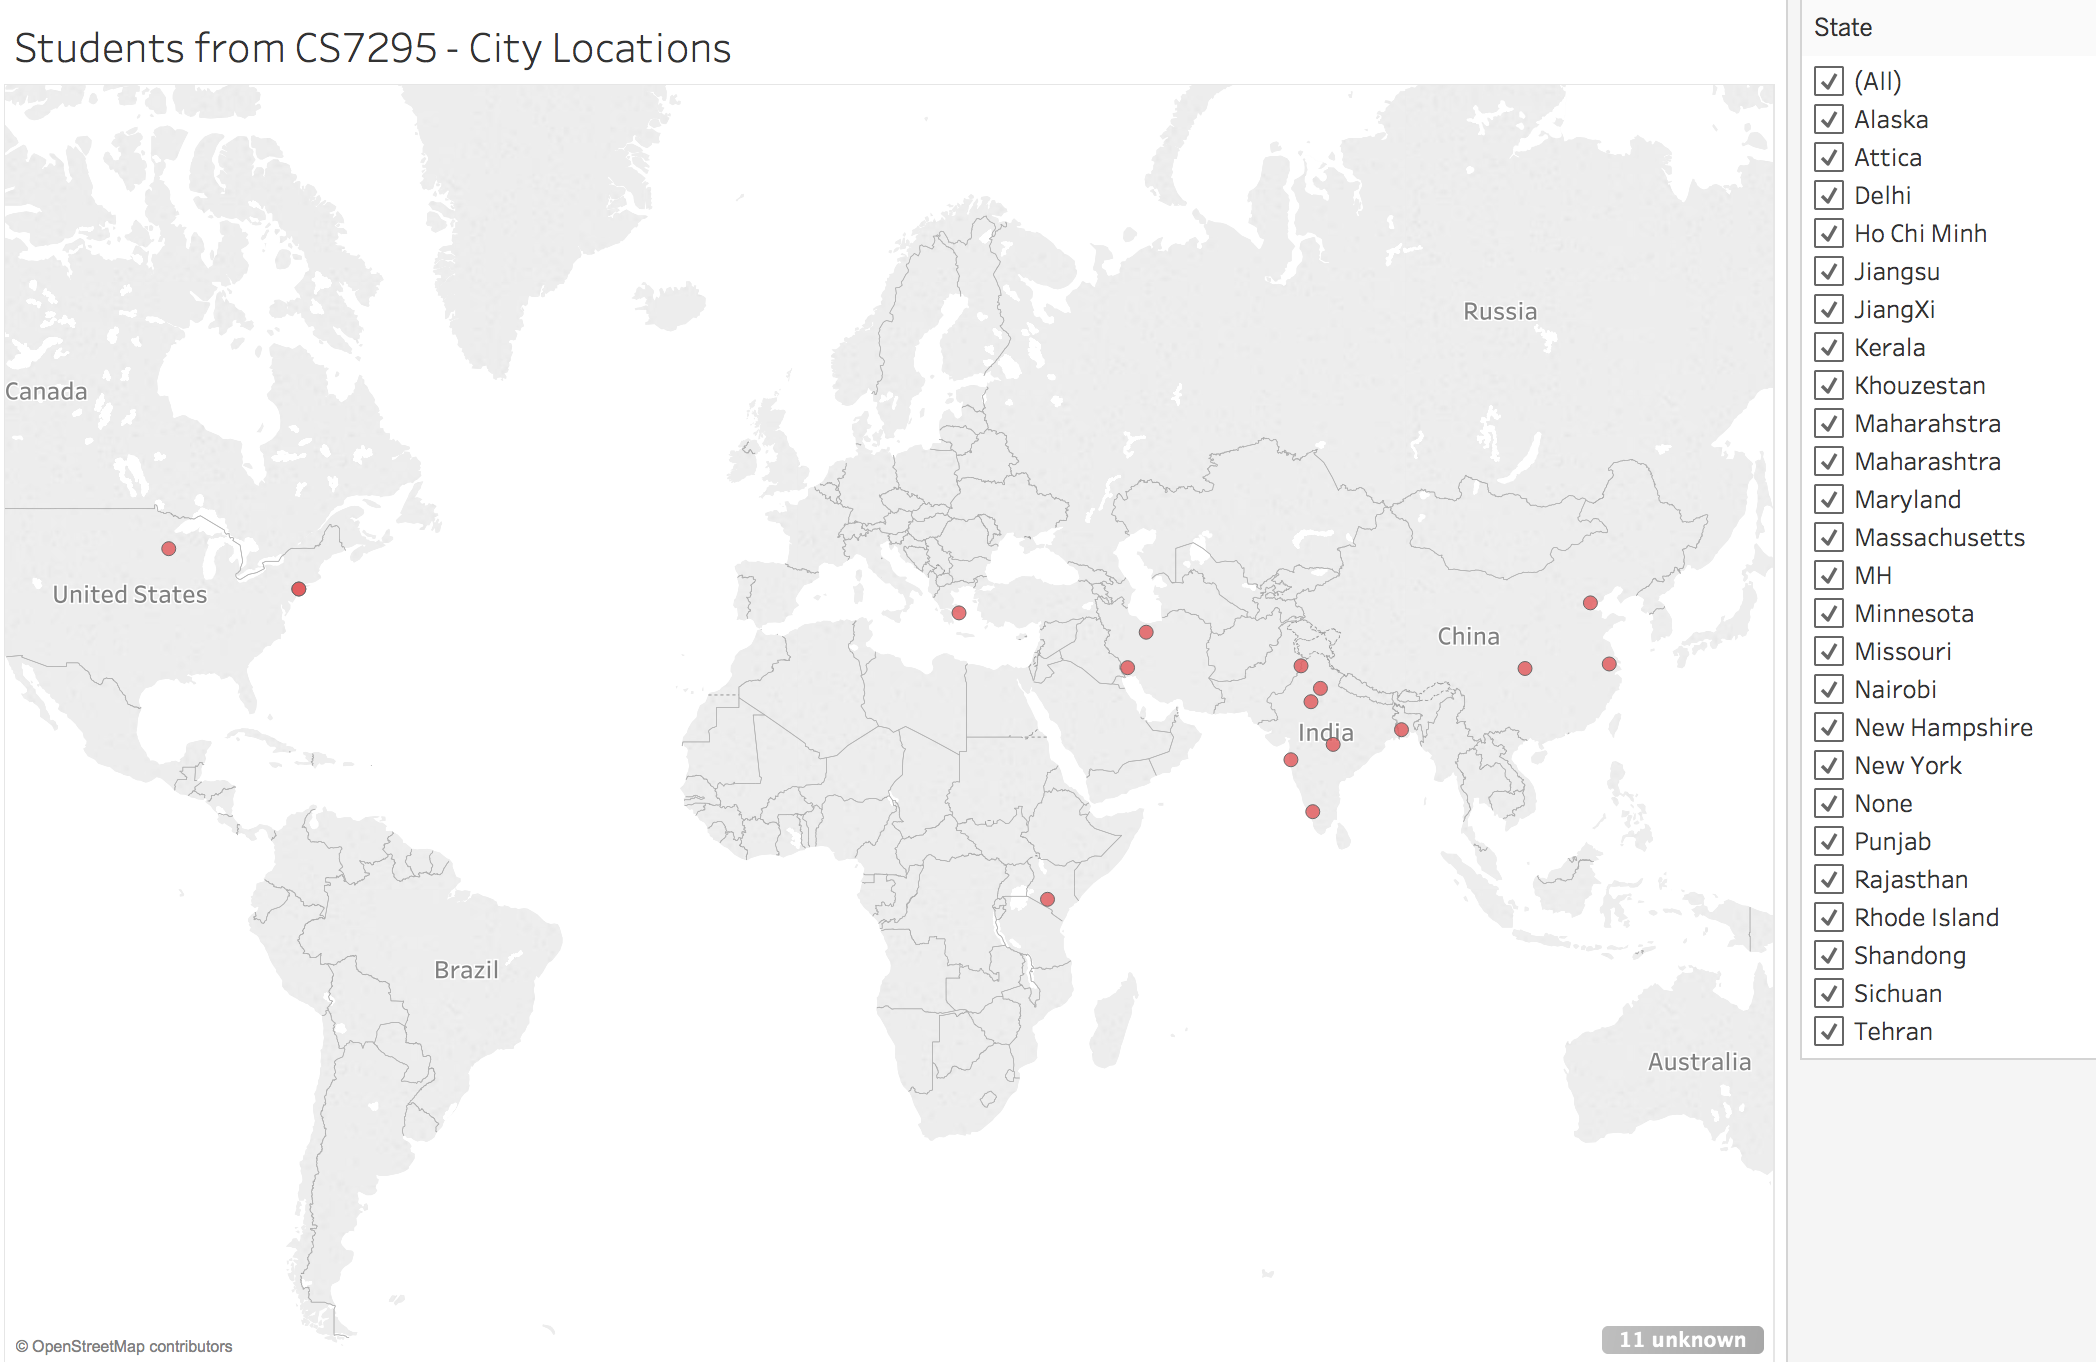
\includegraphics[width=0.7\linewidth]{cities}
}
\end{figure}


\begin{figure}[h]
\centering
{
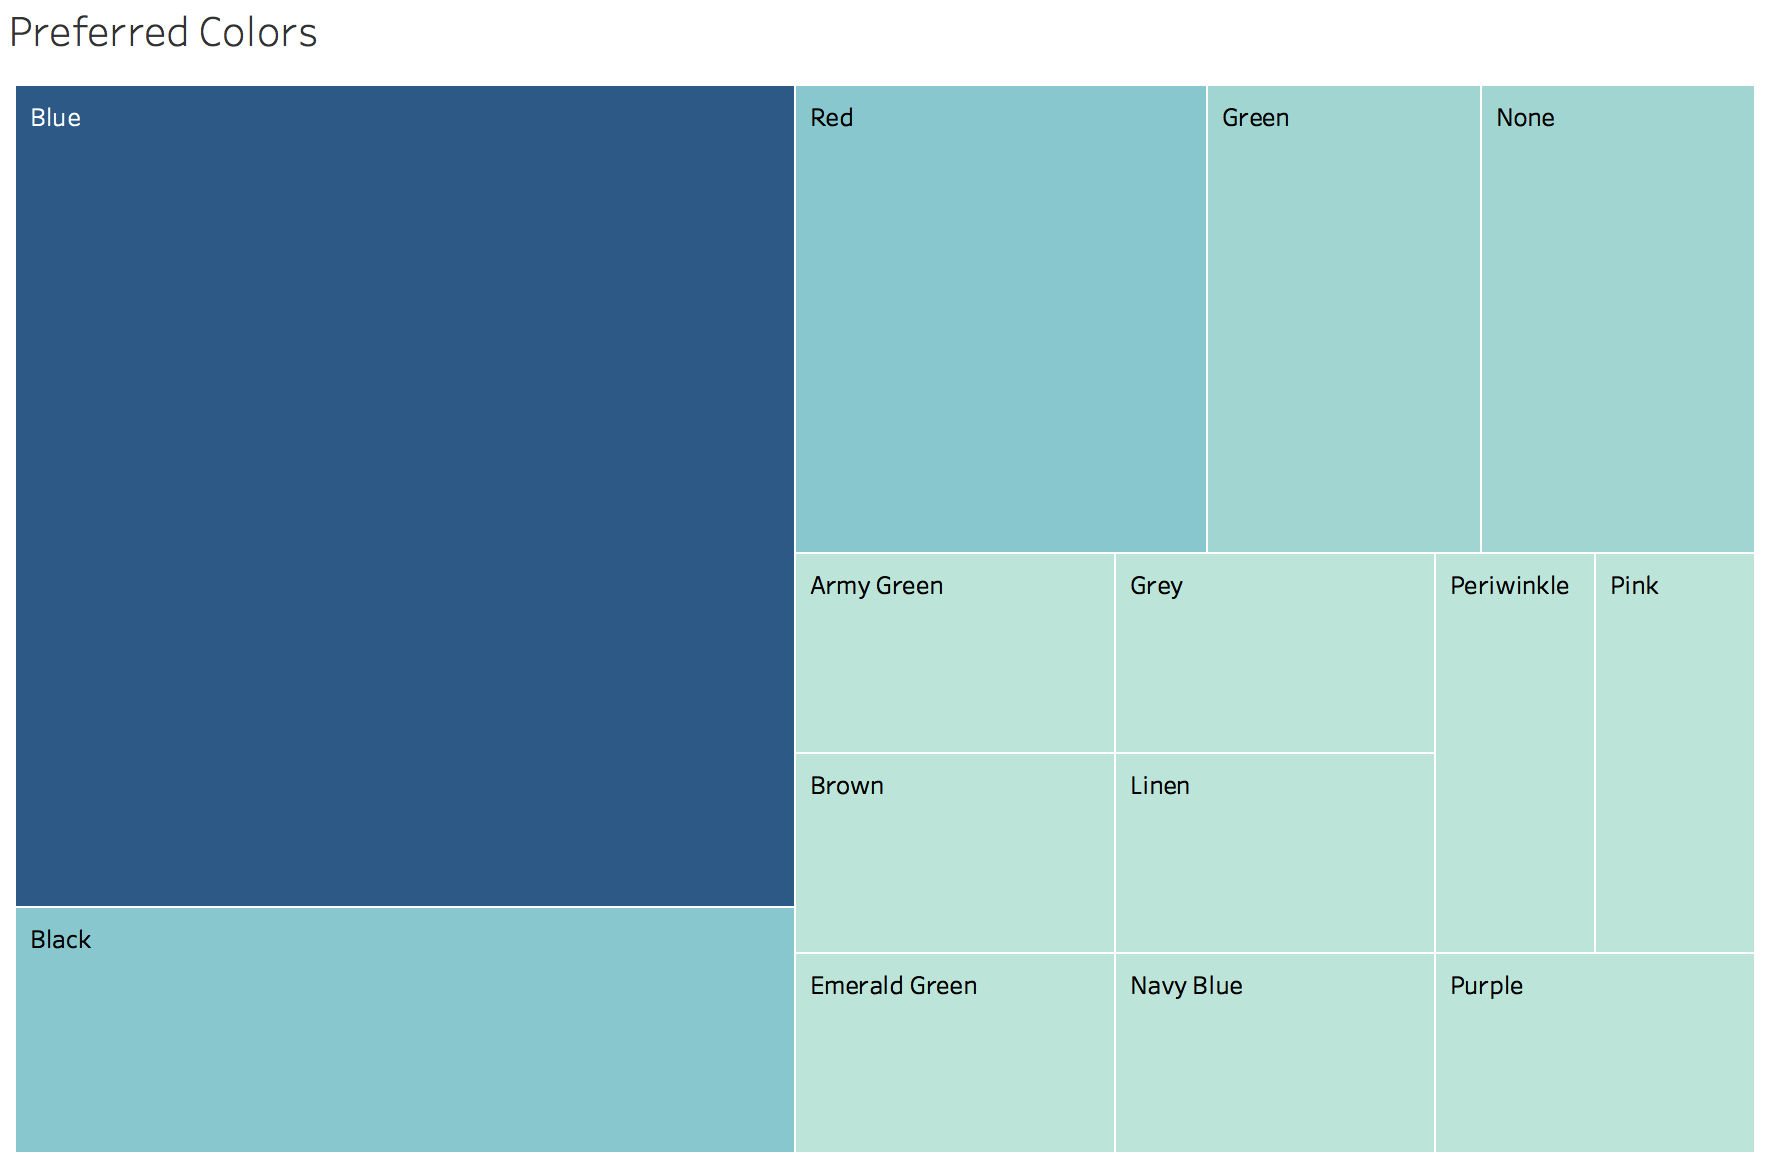
\includegraphics[width=0.7\linewidth]{colors}
}
\end{figure}

\begin{figure}[h]
\centering
{
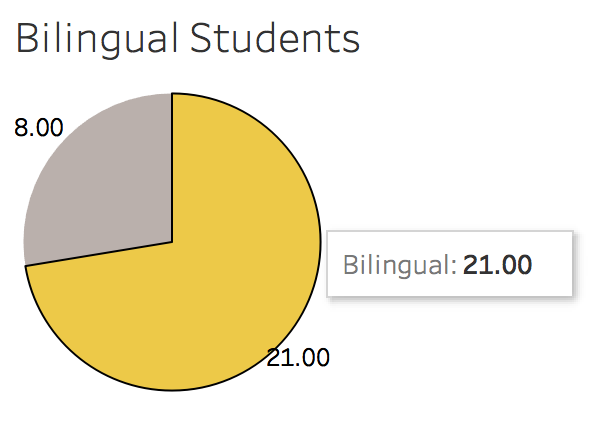
\includegraphics[width=0.4\linewidth]{languages}
}
\end{figure}


\end{document}
